\subsection{SuperCon3D -  Inverse Crystal Structure Generation}
{{\footnotesize
\noindent SuperCon3D introduces 3D crystal structures with associated critical temperatures (Tc) and two deep-learning models: SODNet (equivariant graph model) and DiffCSP-SC (diffusion generator) designed to screen and synthesize high-Tc candidates .


\begin{description}[labelwidth=4cm, labelsep=1em, leftmargin=4cm, itemsep=0.1em, parsep=0em]
  \item[date:] 2024-12-13
  \item[version:] v1.0
  \item[last\_updated:] 2024-12
  \item[expired:] unknown
  \item[valid:] yes
  \item[valid\_date:] 2024-12-13
  \item[url:] \href{https://neurips.cc/virtual/2024/poster/97553}{https://neurips.cc/virtual/2024/poster/97553}
  \item[doi:] unknown
  \item[domain:]
    - Materials Science
  \item[focus:] Dataset and models for predicting and generating high-Tc superconductors using 3D crystal structures
  \item[keywords:]
    - superconductivity
    - crystal structures
    - equivariant GNN
    - generative models
  \item[licensing:] unknown
  \item[task\_types:]
    - Regression (Tc prediction)
    - Generative modeling
  \item[ai\_capability\_measured:]
    - Structure-to-property prediction
    - structure generation
  \item[metrics:]
    - MAE (Tc)
    - Validity of generated structures
  \item[models:]
    - SODNet
    - DiffCSP-SC
  \item[ml\_motif:]
    - Generative
  \item[type:] Dataset + Models
  \item[ml\_task:]
    - Regression, Generation
  \item[solutions:] 0
  \item[notes:] Demonstrates advantage of combining ordered and disordered structural data in model design .

  \item[contact.name:] Zhong Zuo
  \item[contact.email:] unknown
  \item[results.links.name:] ChatGPT LLM
  \item[fair.reproducible:] Yes
  \item[fair.benchmark\_ready:] Yes
  \item[id:] supercond\_-\_\_inverse\_crystal\_structure\_generation
  \item[Citations:] \cite{neurips2024_c4e3b55e}
\end{description}

{\bf Ratings:} ~ \\

\begin{tabular}{p{0.15\textwidth} p{0.07\textwidth} p{0.7\textwidth}}
\hline
Rating & Value & Reason \\
\hline
dataset & 5 & Dataset contains 3D crystal structures and associated properties; well-curated but
not fully released publicly at this time.
 \\
documentation & 4 & Paper and GitHub provide good metadata and data processing descriptions; tutorials
and user guides could be expanded.
 \\
metrics & 4 & Metrics such as MAE for Tc prediction and validity checks for generated structures
are appropriate and clearly described.
 \\
reference\_solution & 4 & Paper provides model architecture details and some training insights, but no
complete open-source reference implementations yet.
 \\
software & 3 & Baseline models (SODNet, DiffCSP-SC) are described in the paper; however,
fully reproducible code and pretrained models are not publicly available yet.
 \\
specification & 5 & Tasks for regression (Tc prediction) and generative modeling with clear input/output
structures and domain constraints are well defined.
 \\
\hline
\end{tabular}

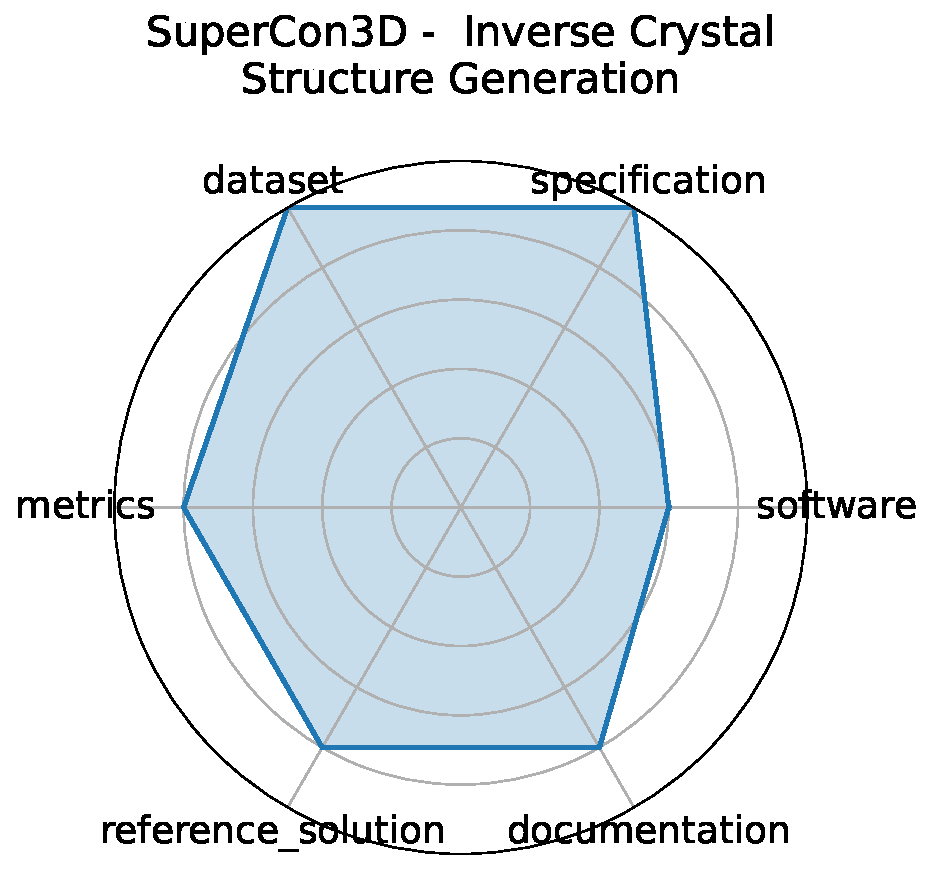
\includegraphics[width=0.2\textwidth]{supercond_-__inverse_crystal_structure_generation_radar.pdf}
}}
\clearpage